\documentclass[tikz,border=2pt]{standalone}
\begin{document}
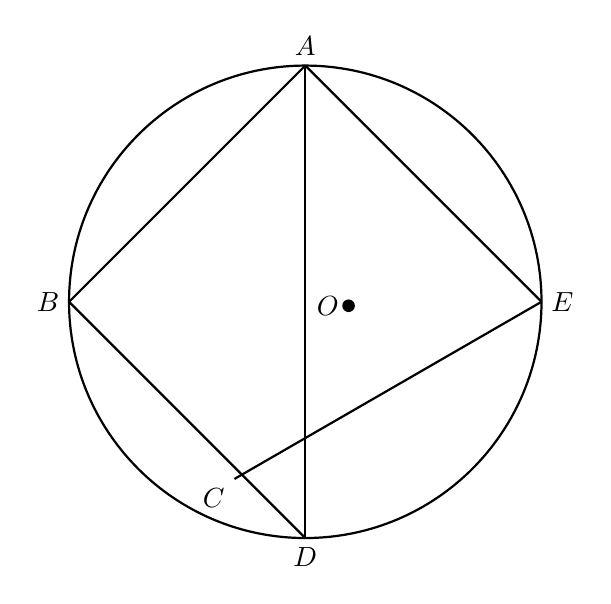
\begin{tikzpicture}[scale=1]

% Circle
\draw[line width=0.8pt] (0,0) circle (3);

% Points on/near the circle
\coordinate (A) at (0,3);
\coordinate (B) at (-3,0);
\coordinate (C) at (-0.9,-2.25);
\coordinate (D) at (0,-3);
\coordinate (E) at (3,0);
\coordinate (O) at (0.55,-0.05);

% Existing segments
\draw[line width=0.8pt] (B) -- (A);
\draw[line width=0.8pt] (A) -- (E);
\draw[line width=0.8pt] (B) -- (D);
\draw[line width=0.8pt] (C) -- (E);

% Added segment AD
\draw[line width=0.8pt] (A) -- (D);

% Point O
\fill (O) circle (0.08);

% Labels
\node[above] at (A) {$A$};
\node[left] at (B) {$B$};
\node[below left] at (C) {$C$};
\node[below] at (D) {$D$};
\node[right] at (E) {$E$};
\node[left] at (O) {$O$};

\end{tikzpicture}
\end{document}
